\documentclass[
	A4paper,
	DIV=9,
	BCOR7mm,
	smallheadings,
	headinclude,
	footinclude,
	headsepline,
	parindent,
	german,
	captions=tableheading,
	abstracton
	]{scrreprt}
\usepackage{blindtext}
\usepackage[ngerman]{babel}
\usepackage[T1]{fontenc}
\usepackage[utf8]{inputenc}
\usepackage{lmodern}
\usepackage{microtype}
\usepackage{geometry}
\usepackage{graphicx}
\usepackage{amssymb}
\usepackage{xcolor}
\usepackage{hyperref}
\hypersetup{
		colorlinks	= true,
		linkcolor	= blue,
		urlcolor	= blue,
		citecolor	= blue,
		pdftitle    = {},
  		pdfsubject  = {},
  		pdfauthor   = {Panagiota Sismanidou},
  		pdfkeywords = {} ,
  		pdfcreator  = {pdflatex},
  		pdfproducer = {LaTeX with hyperref}
	}
\usepackage[style=apa]{biblatex}
\bibliography{Literaturverzeichnis}


\title{Enterprise Architecture Management}
\author{Panagiota Sismanidou}
\date{30.08.2018}

\begin{document}
\maketitle

\tableofcontents

\chapter{Theorie}
\section{Unterpunkt 1}
%%%%
Bis zu vorherigem Zeitpunkt erforderten Computermanipulationsverfahren keine derart ausgefeilten Managementstrategien. Heute implementieren Unternehmen neue Technologien, um die Struktur von Unternehmen zu organisieren und einen strategischen Vorteil zu erlangen, weil diese Verfahren im Laufe der Zeit immer komplexer werden.	
In der ersten Phase der Business-Integration und IT (ab Mitte der 80er Jahre bis Mitte der 90er Jahre) war es unmöglich, die Automatisierung von Geschäftsprozessen zu realisieren, die auch in der Vor-Computer-Ära existierte.
Die zweite Phase (von Mitte der 1990er bis Mitte der 2000er Jahre) ist die Neuorganisation von Geschäftsprozessen. Es wurde davon ausgegangen, dass die Architekten des Informationssystems eine neue Geschäftsorganisationsstruktur anbieten würden, die mit der IT so kompatibel wie möglich ist. Dieser Zeitraum fiel mit der Begeisterung für ERP-Systeme und Geschäftsprozessmodellierungswerkzeuge zusammen.
In diesem Zeitraum, in den neue Produkte und Anwendungen  nehmen Platz auf dem Markt, steigen die Anforderungen an die Anpassungsfähigkeit von Unternehmen jedes Jahr. Es besteht die Notwendigkeit für viele makroökonomische Indikatoren zu einer noch umfassenderen Konsolidierung der verschiedenen  Bereiche eines Unternehmens oder einer Organisation durch den Einsatz elektronischer Werkzeuge.
Als eine Lösung für das Problem der Anpassungsfähigkeit neuer Technologien in der Struktur eines Unternehmens ist das Enterprise Architecture Management (EAM). EnterpriseArchitecture Management hilft dabei, alle Funktionen innerhalb der Organisation zu synchronisieren und initiiert gleichzeitig einen Zyklus kontinuierlicher Änderungen für die Zwecke der Geschäftsoptimierung.
Es gibt keine einheitliche Definition in der Literatur, denn jeder Autor beschreibt die Bedeutung des EAM anders. Eine sehr hilfreiche Definition die ausführlich die Beschreibung des EAM dokumentiert ist folgende:
„Enterprise Architecture Management (EAM) ist ein systematischer und ganzheitlicher Ansatz für das Verstehen, Kommunizieren, Gestalten und Planen der fachlichen und technischen Strukturen im Unternehmen. Es hilft dabei, die Komplexität der IT-Landschaft zu beherrschen und die IT-Landschaft strategisch und businessorientiert  weiterzuentwickeln.“ \autocite{Hanschke2016}
EAM ist ein wesentlicher Bestandteil des strategischen IT-Managements und beinhalten alle Prozesse für die Dokumentation, Analyse, Qualitätssicherung, Planung und Steuerung der Weiterwicklung der IT-Landschaft und der Geschäftsarchitektur.
Es stellte sich jedoch heraus, dass das moderne Geschäft eine sehr mobile Struktur darstellt und sich ständig verändern muss, um seine Position auf dem Markt zu halten.
EAM findet sich hauptsächlich in großen Organisationen - je großer ein Unternehmen ist, desto komplexer ist die IT-Infrastruktur. Darüber hinaus sind große Unternehmen auf einem höheren Niveau der Reife angeordnet sein neigen (basierend Reifemodell des Unternehmens von der Carnegie Mellon University vorgeschlagen) und Einführung von Managementsystemen Architektur stellt das höchste Niveau der Reife. 
%%%%

\blindtext[2]{}\autocite{:Aydin_2009}

\blindtext[2]{}\autocite{:Wintermantel_Medizintechnik}

\blindtext[1]{}\autocite{:Muelhardt_2013}
\section{Unterpunkt 2}
\blindtext[1]{}

\blindtext[2]{}

\blindtext[2]{}

\blindtext[1]{}
\chapter{Fallstudien}
\section{Unterpunkt 1}


\blindtext[1]{}\autocite{:Geschwinde_Rauschdrogen}

\blindtext[2]{}\blindtext[1]{}\autocite{:Muelhardt_2013}
\begin{figure}[htbp]
\begin{center}
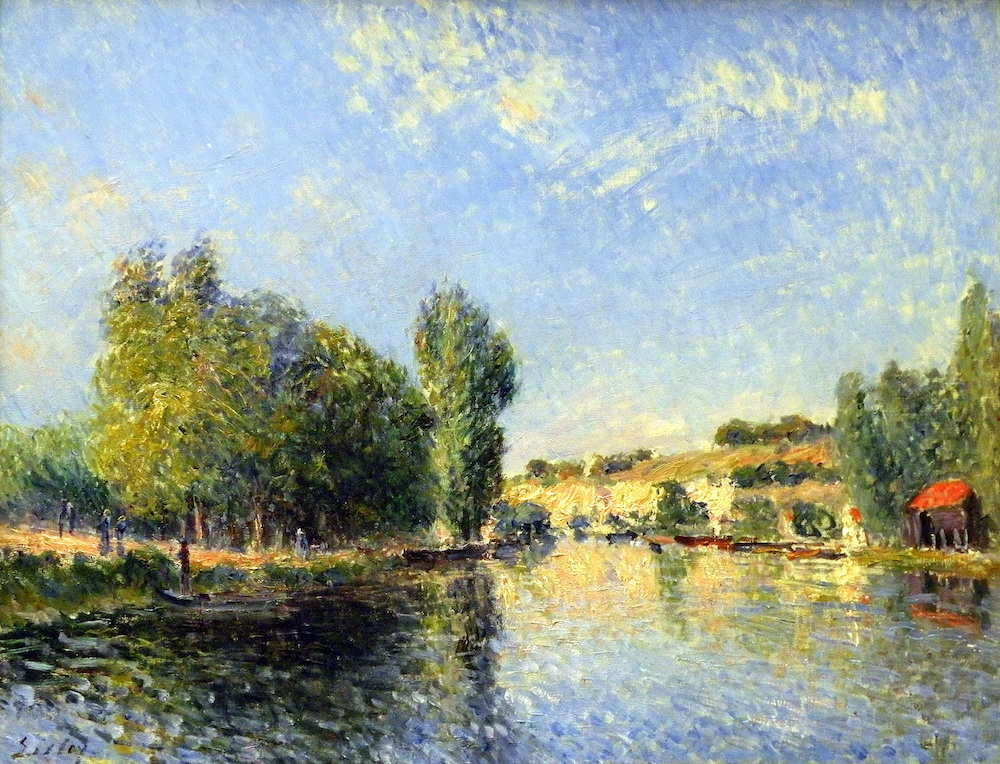
\includegraphics[width=0.7\textwidth]{Abbildungen/Bild1.jpg}
\caption{Bild 1}
\label{fig:Bild1}
\end{center}
\end{figure}

\blindtext[2]{}\autocite{:Wintermantel_Medizintechnik}
\begin{figure}[htbp]
\begin{center}
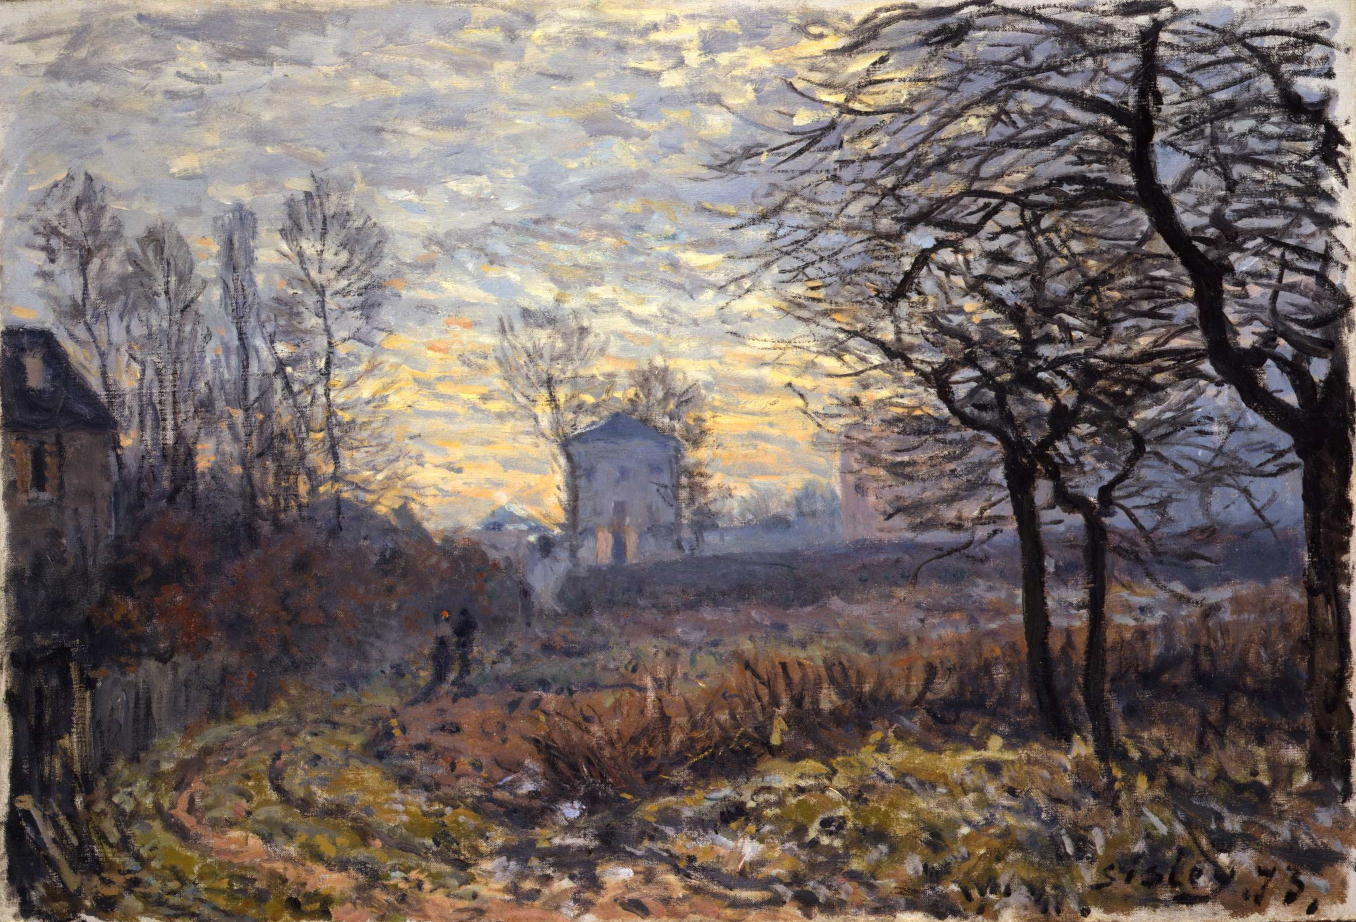
\includegraphics[width=0.7\textwidth]{Abbildungen/Bild2.jpg}
\caption{Bild 2}
\label{fig:Bild2}
\end{center}
\end{figure}

\blindtext[1]{}\autocite{:Keshk_2014}
\section{Unterpunkt 2}
\blindtext[1]{}\autocite{:Aydin_2009}

\blindtext[1]{}\autoref{fig:Bild3}
\blindtext[1]{}\autocite{:Muelhardt_2013}
\begin{figure}[htbp]
\begin{center}
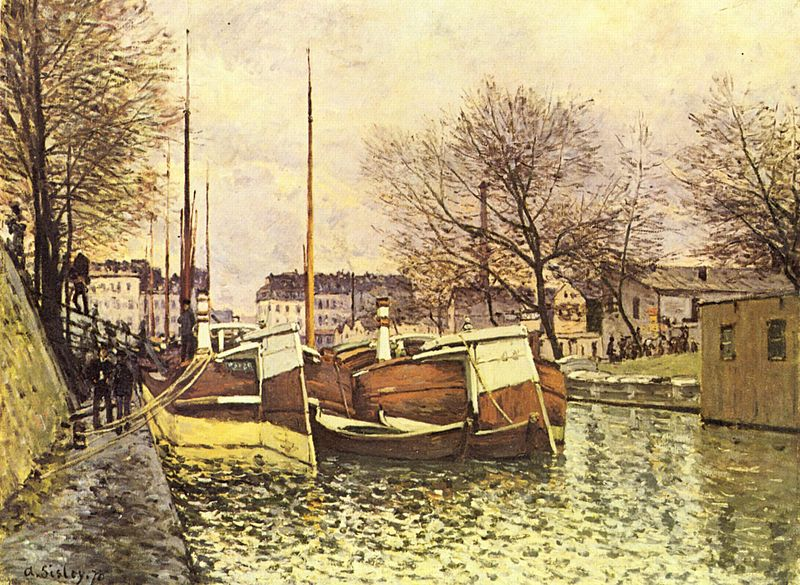
\includegraphics[width=0.7\textwidth]{Abbildungen/Bild3.jpg}
\caption{Bild 3}
\label{fig:Bild3}
\end{center}
\end{figure}

\blindtext[2]{}\autocite{:Geschwinde_Rauschdrogen}
\begin{figure}[htbp]
\begin{center}
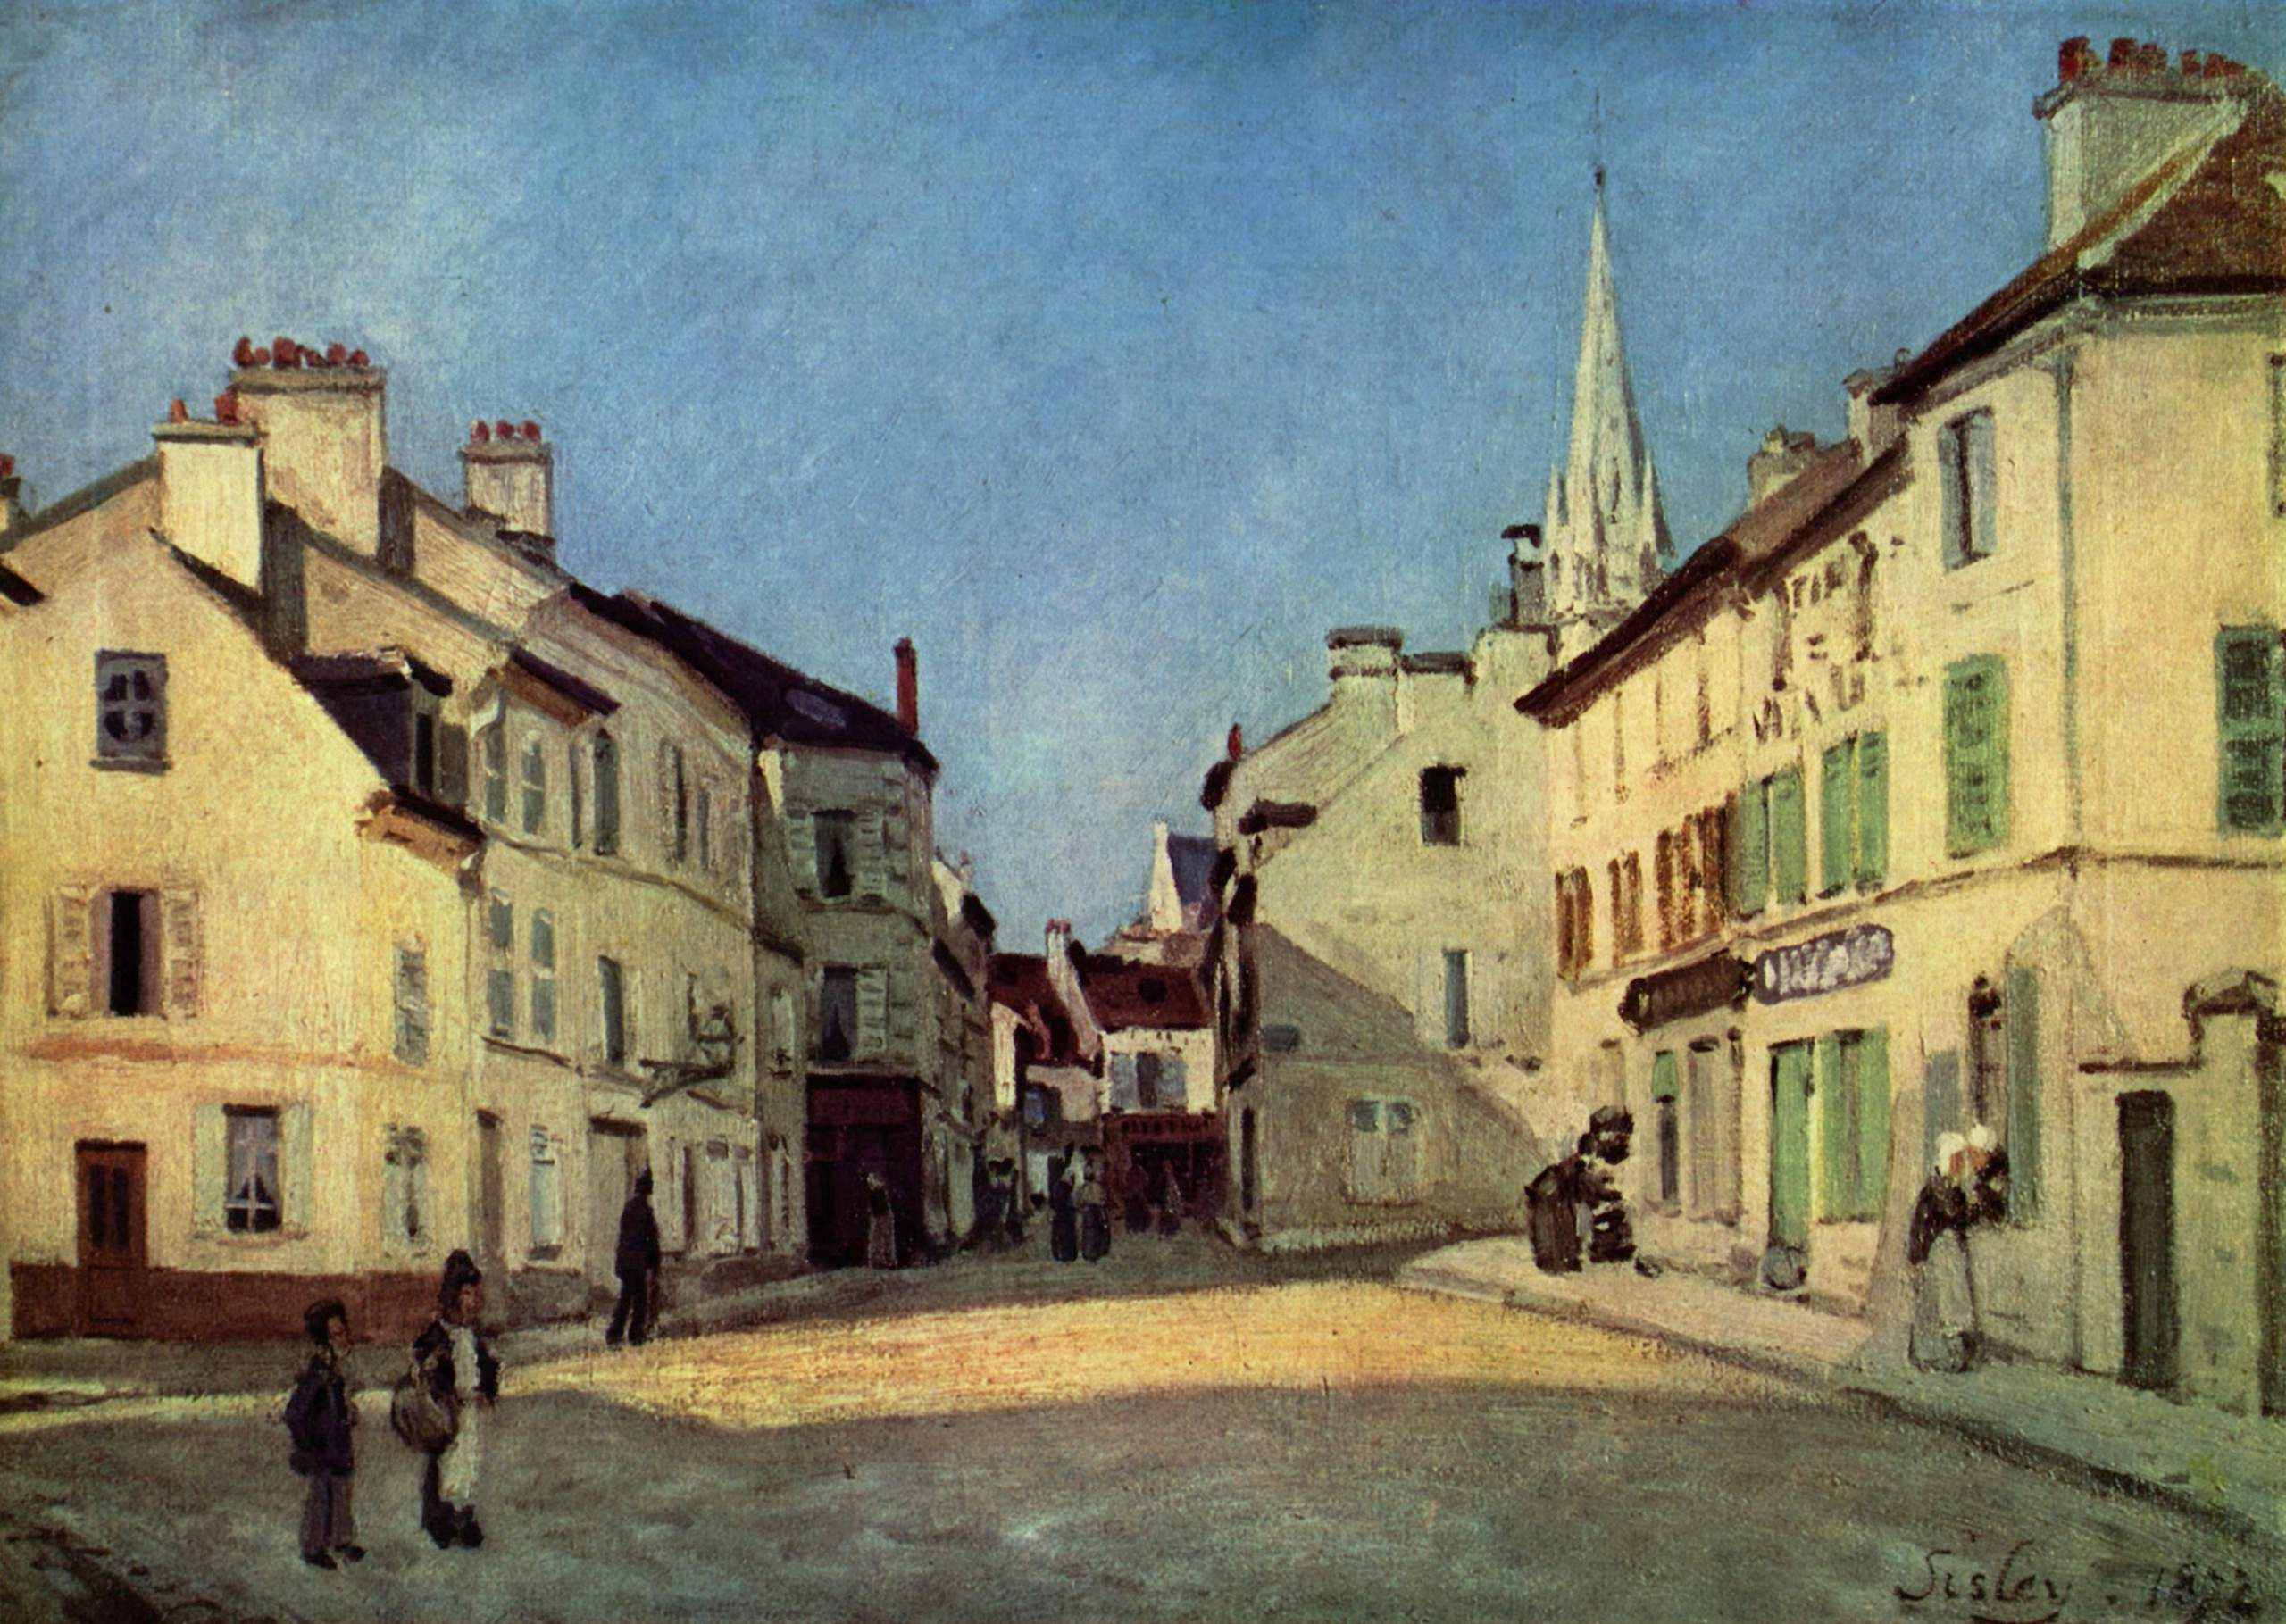
\includegraphics[width=0.7\textwidth]{Abbildungen/Bild4.jpg}
\caption{Bild 4}
\label{fig:Bild4}
\end{center}
\end{figure}

\blindtext[1]{}
\begin{table}[]
\caption{tab:Tabelle}
\begin{center}
\begin{tabular}{|c|c|}
\hline
bla & bla \\
\hline
\hline
bla & bla \\
bla & bla \\
bla & bla \\
bla & bla \\
\hline
\end{tabular}
\end{center}
\label{default}
\end{table}%

\chapter{Fazit}
\blindtext[1]{}

\blindtext[2]{}

\blindtext[2]{}

\blindtext[1]{}

\printbibliography

\end{document}  